\documentclass[french]{article}
\usepackage{amsmath}
\usepackage{amssymb}	% packages that allow mathematical formatting
\usepackage{graphicx}	% package that allows you to include graphics
\usepackage{setspace}	% package that allows you to change spacing
\usepackage{fullpage}	% package that specifies normal margins
\usepackage{microtype}
\usepackage{amsthm}
\newcommand{\argmin}{\operatornamewithlimits{argmin}}
\newcommand{\argmax}{\operatornamewithlimits{argmax}}
\usepackage{listings}
\usepackage{color}
\usepackage{caption}
\usepackage{subcaption}
\usepackage{rotating} % Rotating table
\usepackage{enumerate}
\usepackage{graphicx}               % Necessary to use \scalebox
\usepackage{amsmath,amssymb}

\definecolor{codegreen}{rgb}{0,0.6,0}
\definecolor{codegray}{rgb}{0.5,0.5,0.5}
\definecolor{codepurple}{rgb}{0.58,0,0.82}
\definecolor{backcolour}{rgb}{0.95,0.95,0.95}



\lstdefinestyle{mystyle}{
	backgroundcolor=\color{backcolour},   
	commentstyle=\color{codegreen},
	keywordstyle=\color{blue},
	numberstyle=\tiny\color{codegray},
	stringstyle=\color{codepurple},
	basicstyle=\ttfamily\footnotesize,
	breakatwhitespace=false,         
	breaklines=true,                 
	captionpos=b,                    
	keepspaces=true,                 
	numbers=none,                    
	numbersep=5pt,                  
	showspaces=false,                
	showstringspaces=false,
	showtabs=false,                  
	tabsize=2,
	otherkeywords={!,!=,~,*,\&,\%/\%,\%*\%,\%\%,<-,<<-,/}
}\lstset{style=mystyle}

\usepackage[left=2.5cm, right=2.5cm, top=2cm, bottom = 3cm]{geometry}


\lstdefinestyle{mystyle}{
	backgroundcolor=\color{backcolour},   
	commentstyle=\color{codegreen},
	keywordstyle=\color{blue},
	numberstyle=\tiny\color{codegray},
	stringstyle=\color{codepurple},
	basicstyle=\ttfamily\footnotesize,
	breakatwhitespace=false,         
	breaklines=true,                 
	captionpos=b,                    
	keepspaces=true,                 
	numbers=none,                    
	numbersep=5pt,                  
	showspaces=false,                
	showstringspaces=false,
	showtabs=false,                  
	tabsize=2,
	otherkeywords={!,!=,~,*,\&,\%/\%,\%*\%,\%\%,<-,<<-,/}
}\lstset{style=mystyle}


\begin{document}
\noindent Patrick Shultz\\
Mehra and Prescott

\paragraph{1}
The economy consists of a representative agent with preferences:
\begin{equation*}
	U(c) = E_0 \sum_{t=0}^{\infty}\beta^tu(c_t), \quad u(c) = \frac{c^{1-\alpha}}{1-\alpha}
\end{equation*}
There is no production. Aggregate endowment each period follows the stochastic process
\begin{equation*}
	y_{t+1} = \lambda_{t+1}y_t
\end{equation*}
where the growth rate $\lambda$ takes on one of two value, $\lambda_1$ or $\lambda_2$, with probabilities given by the first order Markovian transition matrix:
\begin{equation*}
	\Pi = \begin{bmatrix} 
	(1+\rho)/2 & (1-\rho)/2\\(1-\rho)/2 & (1+\rho)/2
	\end{bmatrix}
	=\begin{bmatrix} 
	\phi & 1-\phi\\1-\phi & \phi
	\end{bmatrix}
\end{equation*}
Let $\lambda_1=\mu + \sigma$, and $\lambda_2 = \mu-\sigma$. In equilibrium $y_t = c_t$. \\

Download Non-durable and service consumption data from WRDS. Generate real-per capita consumption growth for two sample (a) one that starts at 1929, (b) one that starts at 1950. 

Mehra and Prescott find $0.018$, $0.036$, and $-0.14$, are the mean, standard deviation and autocorrelation of continuous mean consumption growth in their sample, respectively. We can then calculate the parameters of the Markov process as follows:
\begin{itemize}
	\item \textbf{Persistence:} To compute the persistence of the process, consider the indicator function, denoted as  $\xi_t$, which is equal to $1$ in the high growth state and zero otherwise.  Given our transition matrix $\Pi$, we then have 
	\begin{equation*}
	\begin{bmatrix}
	\xi_{t}\\ 1- \xi_t
	\end{bmatrix} = \begin{bmatrix} 
	\phi & 1-\phi\\1-\phi & \phi
	\end{bmatrix} \begin{bmatrix}
	\xi_{t-1}\\ 1- \xi_{t-1}
	\end{bmatrix}
	+
	\begin{bmatrix}
	v_{1, t}\\ v_{2, t}
	\end{bmatrix}
	\end{equation*}
	which implies $\xi_{t+1} = (1-\phi) + \xi_t(\phi -1 +\phi) + v_{1, t+1}$. Taking the unconditional expectation implies the persistence in the process is given by $2\phi -1 = 2(\frac{1}{2}(1+\rho))-1 = \rho$. Thus, $2\phi -1 = -0.014$, and $\phi = 0.43$. Further note that $E\left[\xi_{t+1}\right] = \frac{1-\phi}{2(1-\phi)}$. Thus, the unconditional probability $\pi_1 = \pi_2 = 0.5$. 
	\item\textbf{Mean:} Given that the mean gross growth rates in the high and low growth regimes are given by $\mu + \sigma$ and $\mu -\sigma$, we know that the unconditional mean is given by $\mu = 1.018$.
	\item \textbf{Standard Deviation:} Once again using the unconditional probability derived above, we have that the unconditional variance of the process is given by	$\sigma^2 = 0.5 \sigma^2 + 0.5\sigma^2$, which implies $\sigma = 0.036$. 
\end{itemize}



%-------------------------------------------------------------------------------
% Markov chain calculations 
%-------------------------------------------------------------------------------


\paragraph{a) Markov Chains}
\begin{enumerate}[I.]
	\item Compute the conditional moments of the Markov chain which describes the evolution of the  $\lambda$ process.\\
	
	 Letting $s_t = h/l$ denote whether we are currently in the high or low state, the conditional means are given by
	\begin{equation*}
		\begin{split}
		E\left[\lambda_{t+1}|s_t = h\right] &= \pi_{hh}\lambda_h + \pi_{hl}\lambda_l \\
		&= \phi(\mu + \sigma) + (1-\phi)(\mu-\sigma)\\
		&= \mu + \sigma\rho\\
		E\left[\lambda_{t+1}|s_t = l\right]&=\pi_{lh}\lambda_h + \pi_{ll}\lambda_l \\
		&= (1-\phi)(\mu + \sigma) + \phi(\mu-\sigma)\\
		&= \mu -\sigma\rho\\
		\end{split}
	\end{equation*}
	The conditional variance is generally given by 
	\begin{equation*}
	\begin{split}
		Var(\lambda_{t+1}|s_t=i)&=E\left[\lambda_{t+1}^2|s_t = i\right] - E\left[\lambda_{t+1}|s_t = i\right]^2\\
		&= \sum_j \pi_{ij} \lambda_j^2 - \left(\sum_j \pi_{ij}\lambda_j\right)^2
	\end{split}
	\end{equation*}
	Thus, we have 
	\begin{equation*}
	\begin{split}
		Var(\lambda_{t+1}|s_t = h) &= \pi_{hh}\lambda_h^2 + \pi_{hl}\lambda_l^2 - (\pi_{hh}\lambda_h + \pi_{hl}\lambda_l)^2\\
		&= \phi(\mu + \sigma)^2 + (1-\phi)(\mu-\sigma)^2 + (\phi(\mu + \sigma) - (1-\phi)(\mu-\sigma))^2\\
		&=\sigma^2(\rho^2-1) \\
		Var(\lambda_{t+1}|s_t = l) &=\pi_{lh}\lambda_h^2 + \pi_{ll}\lambda_l^2 - (\pi_{lh}\lambda_h + \pi_{ll}\lambda_l)^2\\
		&= \sigma^2(\rho^2-1)
	\end{split}
	\end{equation*}
	Hence, we see that the conditional variances are equal to each other and the conditional means are different. 
	\item Compute the stationary distribution $\Pi^*$, which satisfies $\Pi^* = \Pi \times \Pi^*$. \\
	
	We know that $\Pi^*\iota = 1$, where $\iota$ denotes the vector of ones. Using these two restrictions, we can solve for $\Pi^*$. Define the matrix $A$ as 
	\begin{equation*}
		A = \begin{bmatrix}
		I_2 - \Pi \\ \iota'
		\end{bmatrix}
	\end{equation*}
	Then we have $A\Pi^* = \left[0\quad0\quad 1\right]'$. The solution for $\Pi^*$ is 
	\begin{equation*}
	\begin{split}
	A\Pi^* &= \left[0\quad0\quad 1\right]'\\
	A'A\Pi^* &= A'\left[0\quad0\quad 1\right]'\\
	\Pi^* &= (A'A)^{-1}A'\left[0 \quad 0 \quad 1\right]'
	\end{split}
	\end{equation*}
	Plugging in our parameters for $\phi$, we get 
	\begin{equation*}
		\Pi^* =	
		\begin{bmatrix}
		0.5\\ 0.5
		\end{bmatrix}
	\end{equation*}
	\item Confirm that the unconditional mean, standard deviation, and first order autocorrelation coeffcient for the $\lambda$ process are $\mu, \sigma$, and $\rho$ respectively. \\
	
	We can calculate the unconditional mean and standard deviation using $\Pi^*$
	\begin{equation*}
		\begin{split}
		E\left[\lambda\right] &= \sum_i \pi_{i}^*\lambda_i\\
		&= 0.5 (\mu+\sigma) + 0.5(\mu -\sigma)\\
		&= \mu\\
		Var(\lambda)&= \sum_i \pi_{i}^* \lambda_i^2 - \left(\sum_i \pi_{i}^*\lambda_i\right)^2\\
		&=0.5 (\mu+\sigma)^2 + 0.5(\mu -\sigma)^2 - (0.5 (\mu+\sigma) + 0.5(\mu -\sigma))^2\\
		&= 0.5( (\mu+\sigma)^2 +(\mu -\sigma)^2) - \mu^2\\
		&=  0.5( 2(\mu^2+\sigma^2)) - \mu^2\\
		& = \sigma^2
		\end{split}
	\end{equation*}
	
	The first order autocorrelation is given by $2\phi -1 = 2((1+\rho)/2)-1 = \rho$. 
	Thus, we have verified that the unconditional mean, standard deviation, and autocorrelation are $\mu$, $\sigma$, $\rho$,  respectively.
\end{enumerate}


%-------------------------------------------------------------------------------
% Term Structure of Interest Rates 
%-------------------------------------------------------------------------------

\paragraph{b) The Term Structure of Interest Rates:} In this economy, like other real economies, an $n$ period bond is a sure claim to a single unit of risk free consumption $n$ periods hence. 

\begin{enumerate}[I.]
	\item Use the agent's first order condition to compute the price $b^1_i$ and the return $R^1_i$, on a one-period bond in each state $i$. Choose $\beta$ to produce a mean real interest rate of $5$ percent (i.e. $R = 1.05$). \\
	
	The first order condition of the investor directly implies the Euler equation
	\begin{equation*}
		b_i^1 = \beta E_t\left[\frac{u'(c_{t+1})}{u'(c_t)}\right] = \beta E \left[(c_{t+1}/c_t)^{-\alpha}\right] = \beta E\left[\lambda_{t+1}^{-\alpha}\right]
	\end{equation*}
	where $\lambda_{t+1}$ is the growth rate in consumption from time $t$ to $t+1$. We can use our Markov chain to compute this expectation, so our general expression for the one period bond price in state $i$ is 
	\begin{equation}
	\begin{split}
		b^1_i = \beta \sum_{j=1}^{N}\pi_{ij}\lambda_j^{-\alpha}
	\end{split}
	\label{eq:bond_price}
	\end{equation}
	Thus, when $i = 1$ (the high state), we have the following bond price
	\begin{equation*}
	\begin{split}
			b^1_1 &= \beta \sum_{j=1}^{N}\pi_{1j}\lambda_j^{-\alpha}\\
			&=\beta \left(\pi_{11}\lambda_1^{-\alpha} + \pi_{12}\lambda_2^{-\alpha}\right)\\
			&=\beta \left(\phi\lambda_1^{-\alpha} + (1-\phi)\lambda_2^{-\alpha}\right)\\
			&= \beta \left(\frac{1+\rho}{2}(\mu+\sigma)^{-\alpha} + \frac{1-\rho}{2}(\mu-\sigma)^{-\alpha}\right)\\
	\end{split}
	\end{equation*}
	Similarly, when $i=2$ (the low state), we have the following bond price 
		\begin{equation*}
	\begin{split}
	b^1_2 &= \beta \sum_{j=1}^{N}\pi_{2j}\lambda_j^{-\alpha}\\
	&=\beta \left(\pi_{21}\lambda_1^{-\alpha} + \pi_{22}\lambda_2^{-\alpha}\right)\\
	&= \beta \left(\frac{1-\rho}{2}(\mu+\sigma)^{-\alpha} + \frac{1+\rho}{2}(\mu-\sigma)^{-\alpha}\right)\\
	\end{split}
	\end{equation*}
	For a one period bond we define the return as $R^1_i = 1/b^1_i$. Using our unconditional probabilities, we then get an the unconditional return as 
	\begin{equation*}
		R^1 = \frac{1}{2}(R^1_1 + R^1_2) = \frac{1}{2\beta}\left(\frac{1}{\frac{1+\rho}{2}(\mu+\sigma)^{-\alpha} + \frac{1-\rho}{2}(\mu-\sigma)^{-\alpha} }+ \frac{1}{\frac{1-\rho}{2}(\mu+\sigma)^{-\alpha} + \frac{1+\rho}{2}(\mu-\sigma)^{-\alpha}}\right)
	\end{equation*}
	We want to find a $\beta$ such that $R^1 = 1.05$, so we solve for a $\beta$ that satisfies
	\begin{equation*}
	\beta =  \frac{1}{2\times 1.05}\left(\frac{1}{\frac{1+\rho}{2}(\mu+\sigma)^{-\alpha} + \frac{1-\rho}{2}(\mu-\sigma)^{-\alpha} }+ \frac{1}{\frac{1-\rho}{2}(\mu+\sigma)^{-\alpha} + \frac{1+\rho}{2}(\mu-\sigma)^{-\alpha}}\right)
	\end{equation*}
	Using $\mu, \sigma, $ and $,\rho$ from our various samples gives the following table\\
	
	\begin{table}[!htbp] \centering 
		\caption{Moments and implied $\beta$ for the various samples} 
		\label{tab:sample_moments} 
		\begin{tabular}{@{\extracolsep{5pt}} ccccc} 
			\\[-1.8ex]\hline 
			\hline \\[-1.8ex] 
			& $\mu$ & $\sigma$ & $\rho$ & implied $\beta$ \\ 
			\hline \\[-1.8ex] 
			Mehra and Prescott & $1.018$ & $0.036$ & $-0.140$ & $0.983$ \\ 
			Full Sample & $1.019$ & $0.032$ & $0.405$ & $0.987$ \\ 
			Post War & $1.019$ & $0.020$ & $0.320$ & $0.988$ \\ 
			\hline \\[-1.8ex] 
			\end{tabular} 
	\end{table}
	Tables throughout the rest of this write up use the above parameterizations. 
	\item Consider the \textit{risk neutral probability} defined by 
	\begin{equation*}
		p_{ij} = \frac{\pi_{ij}\beta \lambda_j^{-\alpha}}{b^1_i}
	\end{equation*}
	where $\pi_{ij}\equiv$the $i, j$ element of $\Pi$. Show that the $p$'s are legitimate probabilities. \\
	
	Substituting in Equation \ref{eq:bond_price}, the risk neutral probabilities are given by 
	\begin{equation*}
	\begin{split}
		p_{ij} &= \frac{\pi_{ij}\beta \lambda_j^{-\alpha}}{\beta \sum_{j=1}^{N}\pi_{ij}\lambda_j^{-\alpha}}\\
		&=\frac{\pi_{ij} \lambda_j^{-\alpha}}{\sum_{j=1}^{N}\pi_{ij}\lambda_j^{-\alpha}}\\
	\end{split}
	\end{equation*}
	The expression after the second equality makes it clear that $\sum_j p_{ij}$ must sum to one.  
	\begin{equation*}
		\sum_j p_{ij} = \sum_j\frac{\pi_{ij} \lambda_j^{-\alpha}}{\sum_{j}\pi_{ij}\lambda_j^{-\alpha}} = \frac{1}{\sum_{j}\pi_{ij}\lambda_j^{-\alpha}}\sum_j \pi_{ij} \lambda_j^{-\alpha} = 1
	\end{equation*}
	where the second equality holds, because once we have summed over all the $j$'s in the denominator, the term is only dependent on $i$. Noting that $p_{ij}$ is clearly less than one and positive (the numerator is the price of a state contingent claim, so it is positive by no arbitrage), so the risk neutral probabilities are in fact legitimate. \\
	
	Show that an asset with dividends $d_j$ in state $j$, one period hence has current value given by 
	\begin{equation*}
		q_i = b^1_i E_p\left[d\right]
	\end{equation*}
	where the expectation is taken with respect to the risk neutral probability measure. \\
	
	First order conditions imply the Euler equation
	\begin{equation*}
	\begin{split}
			q_i &= E_i\left[\beta \lambda_j^{-\alpha}d_j\right]\\
			&= \sum_{j=1}^{N}\pi_{ij} \beta \lambda_j^{-\alpha}d_j\\
			&= \frac{b^1_i}{b^1_i}\sum_{j=1}^{N}\pi_{ij} \beta \lambda_j^{-\alpha}d_j\\
			&= b^1_i\sum_{j=1}^{N}\frac{\pi_{ij} \beta \lambda_j^{-\alpha}d_j}{b^1_i}\\
			&= b^1_i\sum_{j=1}^{N}p_{ij}d_j = b^1_i E_p\left[d\right]\\
	\end{split}
	\end{equation*}
	\item Use the agent's first order conditions or the risk neutral pricing formula to compute prices and expected one period holding returns on a two period bond in each state $i$. \\
	
	Define the expected holding period return in state $i$ as the expected gross return on buying a two period bond today and selling it tomorrow
	\begin{equation*}
	E_i\left[hpr\right]	=E_i\left[\frac{b_{i'}^1}{b^2_i}\right]  = \frac{E_i\left[b_{i'}^1\right]}{b^2_i}
	\end{equation*}
	where the $i'$ is the state we are in tomorrow. \\ 
	First, we solve for the price of a two period bond, $b^2_i$, in each state $i$. Using risk neutral probabilities the price is given by 
	\begin{equation}
	\begin{split}
		b_i^2 &= b_i^1E_p\left[b_j^1\right] = b_i^1 \left[p_{i1}b_1^1+p_{i2}b_2^1 \right] = \\
		&= \left(\beta \sum_{j=1}^{N}\pi_{ij}\lambda_j^{-\alpha}\right)\left[\frac{\pi_{i1} \lambda_1^{-\alpha}}{\sum_{j=1}^{N}\pi_{ij}\lambda_j^{-\alpha}}\left(\beta \sum_{j=1}^{N}\pi_{1j}\lambda_j^{-\alpha}\right) + \frac{\pi_{i2} \lambda_2^{-\alpha}}{\sum_{j=1}^{N}\pi_{ij}\lambda_j^{-\alpha}}\left(\beta \sum_{j=1}^{N}\pi_{2j}\lambda_j^{-\alpha}\right)\right]\\
	\end{split}
	\label{eq:two_period_state_bond_prices}
	\end{equation}
	Thus, in state $1$ the two period bond price is
	\begin{equation*}
		\begin{split}
		b_1^2 & = \left(\beta \sum_{j=1}^{N}\pi_{1j}\lambda_j^{-\alpha}\right)\left[\frac{\pi_{11} \lambda_1^{-\alpha}}{\sum_{j=1}^{N}\pi_{ij}\lambda_j^{-\alpha}}\left(\beta \sum_{j=1}^{N}\pi_{1j}\lambda_j^{-\alpha}\right) + \frac{\pi_{12} \lambda_2^{-\alpha}}{\sum_{j=1}^{N}\pi_{ij}\lambda_j^{-\alpha}}\left(\beta \sum_{j=1}^{N}\pi_{2j}\lambda_j^{-\alpha}\right)\right]\\
		&=\frac{1}{4} \beta ^2 \bigg(\left(1-\rho ^2\right)(\mu -\sigma )^{-2 \alpha }-2 (\rho -1) (\mu+\sigma)^{-\alpha } (\mu -\sigma )^{-\alpha}+(\rho +1)^2 (\mu +\sigma )^{-2 \alpha }\bigg)
		\end{split}
	\end{equation*}
	and in state $2$, the two period bond price is 
	\begin{equation*}
	\begin{split}
	b_2^2 & = \left(\beta \sum_{j=1}^{N}\pi_{2j}\lambda_j^{-\alpha}\right)\left[\frac{\pi_{21} \lambda_1^{-\alpha}}{\sum_{j=1}^{N}\pi_{ij}\lambda_j^{-\alpha}}\left(\beta \sum_{j=1}^{N}\pi_{1j}\lambda_j^{-\alpha}\right) + \frac{\pi_{22} \lambda_2^{-\alpha}}{\sum_{j=1}^{N}\pi_{ij}\lambda_j^{-\alpha}}\left(\beta \sum_{j=1}^{N}\pi_{2j}\lambda_j^{-\alpha}\right)\right]\\
	&=\frac{1}{4} \beta ^2 \bigg(\left(1-\rho^2\right)(\mu +\sigma )^{-2 \alpha }-2 (\rho -1) (\mu +\sigma)^{-\alpha } (\mu -\sigma )^{-\alpha }+(\rho +1)^2 (\mu-\sigma )^{-2\alpha }\bigg)
	\end{split}
	\end{equation*}


 Next, we solve for $E_i\left[b_{i'}^1\right]$. 
 \begin{equation}
 \begin{split}
  	E_i\left[b_{i'}^1\right] &= \sum_{j=1}^2 \pi_{ij}b^1_j=\pi_{i1}b^1_1 + \pi_{i2}b^1_2\\
  	&= \pi_{i1}\beta \sum_{j=1}^{N}\pi_{1j}\lambda_j^{-\alpha} + \pi_{i2}\beta \sum_{j=1}^{N}\pi_{2j}\lambda_j^{-\alpha}\\
  	&= \pi_{i1}\left(\beta \left(\frac{1+\rho}{2}(\mu+\sigma)^{-\alpha} + \frac{1-\rho}{2}(\mu-\sigma)^{-\alpha}\right)\right) + \pi_{i2}\left(\beta \left(\frac{1+\rho}{2}(\mu+\sigma)^{-\alpha} + \frac{1-\rho}{2}(\mu-\sigma)^{-\alpha}\right)\right)
 \end{split}
 \label{eq:expected_bond_price}
 \end{equation}
 Thus, we have 
 \begin{equation*}
 	\begin{split}
 	E_1\left[b^1_{i'}\right] & = \frac{1}{2} \beta \left(\left(\rho^2+1\right) (\mu +\sigma
 	)^{-\alpha }-\left(\rho^2-1\right) (\mu -\sigma)^{-\alpha }\right)\\
 	E_2\left[b^1_{i'}\right] & = \frac{1}{2} \beta \left(\left(\rho^2+1\right) (\mu -\sigma
 	)^{-\alpha }-\left(\rho^2-1\right) (\mu +\sigma)^{-\alpha }\right)\\
 	\end{split}
 \end{equation*}
 Together, Equations \ref{eq:two_period_state_bond_prices} and \ref{eq:expected_bond_price} characterize the expected holding period return in terms of our model parameters. 
 \begin{equation*}
 	\begin{split}
 	E_1\left[hpr\right] &= \frac{E_1\left[b^1_{i'}\right]}{b^2_1}=\frac{2 \left(\left(\rho ^2+1\right) (\mu +\sigma
 		)^{-\alpha }-\left(\rho ^2-1\right) (\mu -\sigma
 		)^{-\alpha }\right)}{\beta  \left(-\left(\rho
 		^2-1\right) (\mu -\sigma )^{-2 \alpha }-2 (\rho -1)
 		(\mu +\sigma )^{-\alpha } (\mu -\sigma )^{-\alpha
 		}+(\rho +1)^2 (\mu +\sigma )^{-2 \alpha }\right)}\\
 	E_2\left[hpr\right] &= \frac{E_2\left[b^1_{i'}\right]}{b^2_2}= \frac{2 \left(\left(\rho ^2+1\right) (\mu -\sigma)^{-\alpha }-\left(\rho ^2-1\right) (\mu+\sigma)^{-\alpha}\right)}{\beta\left(-\left(\rho^2-1\right)(\mu +\sigma )^{-2 \alpha }+(\rho +1)^2(\mu -\sigma )^{-2 \alpha }-2 (\rho -1) (\mu+\sigma)^{-\alpha}(\mu-\sigma)^{-\alpha
 		}\right)}
 	\end{split}
 \end{equation*}
 Thus, we get the following expected holding period returns and bond prices
	\begin{table}[!htbp] \centering 
	\caption{Bond prices and Expected Holding Period Returns} 
	\label{} 
	\begin{tabular}{@{\extracolsep{5pt}} ccccccc} 
		\\[-1.8ex]\hline 
		\hline \\[-1.8ex] 
		& $b^1_1$ & $b^1_2$ & $b^2_1$ & $b^2_2$ & $E_1\left[hpr\right]$& $E_1\left[hpr\right]$\\ 
		\hline \\[-1.8ex] 
		Mehra Prescott & $0.93$ & $0.91$ & $0.85$ & $0.84$ &$1.08$ & $1.10$\\ 
		Full Sample & $0.93$ & $0.97$ & $0.88$ & $0.942$ & 1.07&1.02 \\ 
		Post War Sample & $0.94$ & $0.96$ & $0.89$ & $0.92$ &1.06&1.04\\ 
		\hline \\[-1.8ex] 
		\end{tabular} 
	\end{table} 
 \item \textit{Implied Forward Rates} are a useful way to express the term-structure of interest rates. Define the implied two-period ahead forward rate in state $i$ as 
 \begin{equation*}
 	(1+f_i^{1\to2}) = b^1_i/b^2_i
 \end{equation*}
 We can interpret this expression as the rate an investor can lock in today by shorting the one period bond and buying the the two period bond. There is zero cost of the trade today, at time $1$ you must pay back the one period bond, and at time $2$ you receive the payment from the time-0 $2$ period bond. Thus, it is equivalent to taking a loan from time $1$ to time $2$. 
 I use the following definition of the risk premium on a two year bond 
 
 where $f_i^{1\to2}$ is the forward rate from period $1$ to $2$. Thus, our expression for the risk premium is defined as the difference between the expected future one year spot rate and the implied forward rate over the same investment horizon. Intuitively, $rp$ should be equal to zero, since two ways of getting money from $t=1$ to $t=2$ (either locking in a rate today or waiting then borrowing at $t=1$) should be the same. \\
 
 Using our previously derived expressions for the bond prices, the forward rates are given by
 \begin{equation*}
 	\begin{split}
 	(1+f_1^{1\to2}) &= \frac{\beta \left(\frac{1+\rho}{2}(\mu+\sigma)^{-\alpha} + \frac{1-\rho}{2}(\mu-\sigma)^{-\alpha}\right)}{\frac{1}{4} \beta ^2 \bigg(\left(1-\rho ^2\right)(\mu -\sigma )^{-2 \alpha }-2 (\rho -1) (\mu+\sigma)^{-\alpha } (\mu -\sigma )^{-\alpha}+(\rho +1)^2 (\mu +\sigma )^{-2 \alpha }\bigg)}\\
 	(1+f_2^{1\to2}) &= \frac{\beta \left(\frac{1-\rho}{2}(\mu+\sigma)^{-\alpha} + \frac{1+\rho}{2}(\mu-\sigma)^{-\alpha}\right)}{\frac{1}{4} \beta ^2 \bigg(\left(1-\rho^2\right)(\mu +\sigma )^{-2 \alpha }-2 (\rho -1) (\mu +\sigma)^{-\alpha } (\mu -\sigma )^{-\alpha }+(\rho +1)^2 (\mu-\sigma )^{-2\alpha }\bigg)}\\
 	\end{split}
 \end{equation*}
The risk premium is just the yield on the two-year bond in excess of the risk free rate, which is the yield on the year bond in this model. We can think of this as the additional compensation required to induce risk averse investors to purchase the two period rather than one period bond. Thus, we define the risk premium on the two year bond as $rp_i = R_i^2 - R_i^1 = \frac{1}{\sqrt{b^2_i}} - \frac{1}{b^1_i}$. Thus, we get the following monstrosity of expressions for the risk premium 
\begin{equation*}
	\begin{split}
	rp_1 &=\frac{2}{\sqrt{\beta ^2 \left(-\left(\rho ^2-1\right)
			(\mu -\sigma )^{-2 \alpha }-2 (\rho -1) (\mu
			+\sigma )^{-\alpha } (\mu -\sigma )^{-\alpha
			}+(\rho +1)^2 (\mu +\sigma )^{-2 \alpha
			}\right)}}\\
		&-\frac{2}{\beta  \left((\rho +1) (\mu
		+\sigma )^{-\alpha }-(\rho -1) (\mu -\sigma
		)^{-\alpha }\right)}\\
    rp_2 &=\frac{2}{\sqrt{\beta ^2 \left(-\left(\rho ^2-1\right)
    		(\mu +\sigma )^{-2 \alpha }+(\rho +1)^2 (\mu
    		-\sigma )^{-2 \alpha }-2 (\rho -1) (\mu +\sigma
    		)^{-\alpha } (\mu -\sigma )^{-\alpha
    		}\right)}}\\
    	&-\frac{2}{\beta  \left((\rho +1) (\mu
    	-\sigma )^{-\alpha }-(\rho -1) (\mu +\sigma
    	)^{-\alpha }\right)}\\	
   \end{split}
\end{equation*}
Thus, we get the following forward rates and risk premiums 
	\begin{table}[!htbp] \centering 
	\caption{Forward Rates and Risk Premiums} 
	\label{tab:forward_rates} 
	\begin{tabular}{@{\extracolsep{5pt}} ccccccc} 
		\\[-1.8ex]\hline 
		\hline \\[-1.8ex] 
		& $1+f_1$ & $1+f_2$ & $rp_1$ & $rp_2$ \\ 
		\hline \\[-1.8ex] 
		Mehra Prescott & $1.089$ & $1.086$ & $0.006$ & $-0.006$\\ 
		Full Sample & $1.05$ & $1.04$ & $-0.009$ & $0.007$ \\ 
		Post War Sample & $1.05$ & $1.04$ & $-0.005$ & $0.004$ \\ 
		\hline \\[-1.8ex] 
	\end{tabular} 
\end{table} \\
 The expectations hypothesis is 
 \begin{equation}
 1+f_i^{1\to2} = E_i\left[R^1_{i'}\right] + rp_i
 \label{eq:EH}
 \end{equation} 
 When the risk premiums are zero, the forward rate is an unbiased predictor of the one year interest rate one year ahead. The final two columns of Table \ref{tab:forward_rates} two columns show that in this model, the expectations hypothesis nearly holds. 
 \item \textit{Sensitivity of Risk Premium to parameters}\\
 In Figure \ref{fig:risk_premium_alpha}, we see how the risk premium responds to various values of $\alpha$ for the parameters of our different samples. We see that with low levels of $\alpha$ the risk premium is near zero. As we increase risk aversion, the risk premium also increases, and eventually starts to decrease. \\
 \begin{figure}[!htb]
 	\centering
 	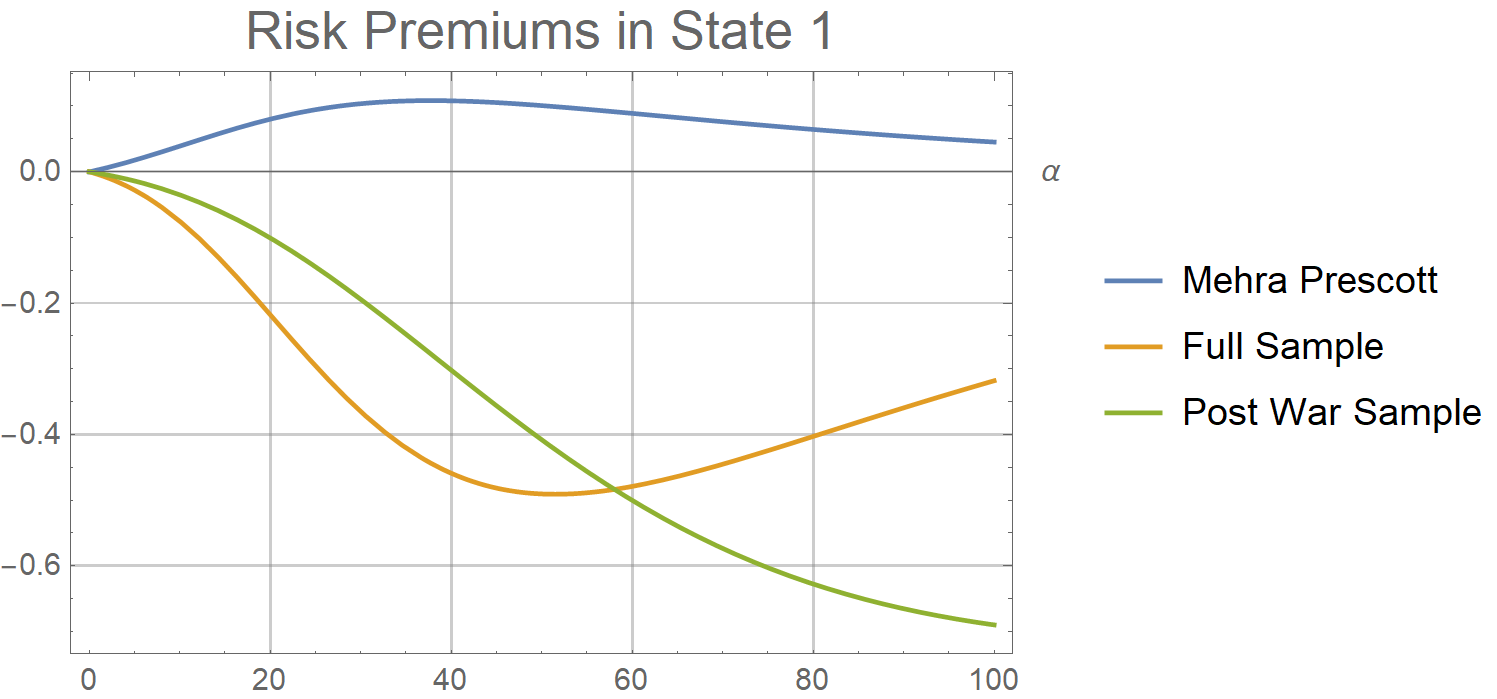
\includegraphics[width=0.75\textwidth]{risk_premium_alpha.png}
 	\caption{Sensitivity of risk premium to $\alpha\in\left[0, 100\right]$ for our various samples.}
 	 	\label{fig:risk_premium_alpha}
 \end{figure}

 \begin{figure}[!htb]
	\centering
	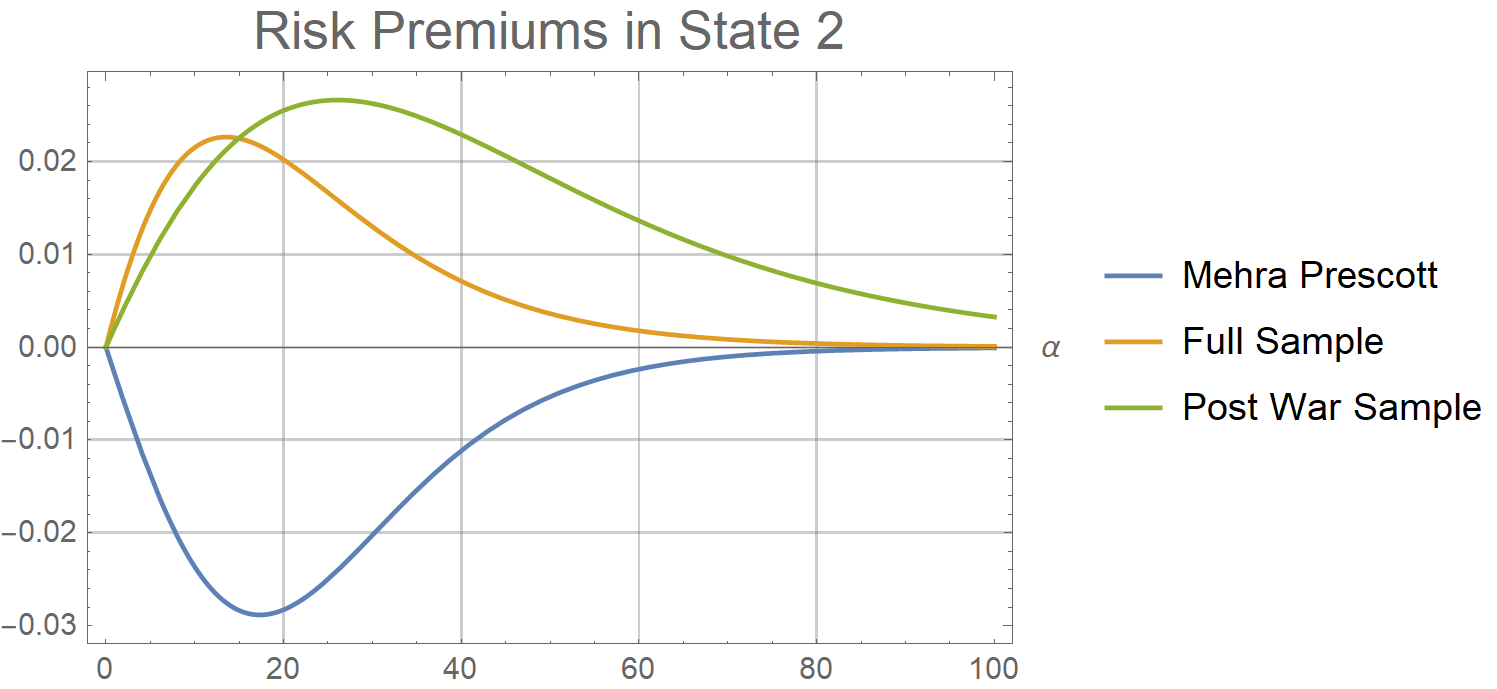
\includegraphics[width=0.75\textwidth]{risk_premium_alpha_2.png}
	\caption{Sensitivity of risk premium to $\alpha\in\left[0, 100\right]$ for our various samples.}
	\label{fig:risk_premium_alpha_2}
\end{figure}
We see a positive risk premium for the non Mehra-Prescott sample periods. Notably, these display a positive rather than negative autocorrelation. We can further investigate this by plotting the Mehra-Prescott parameter implied risk premium with $\alpha = 2$, but varying $\rho$. We see that we need a negative autocorrelation of consumption growth to get a positive risk premium, however we know that consumption growth has been positively autocorrelated. 
  \begin{figure}[!htb]
 	\centering
 	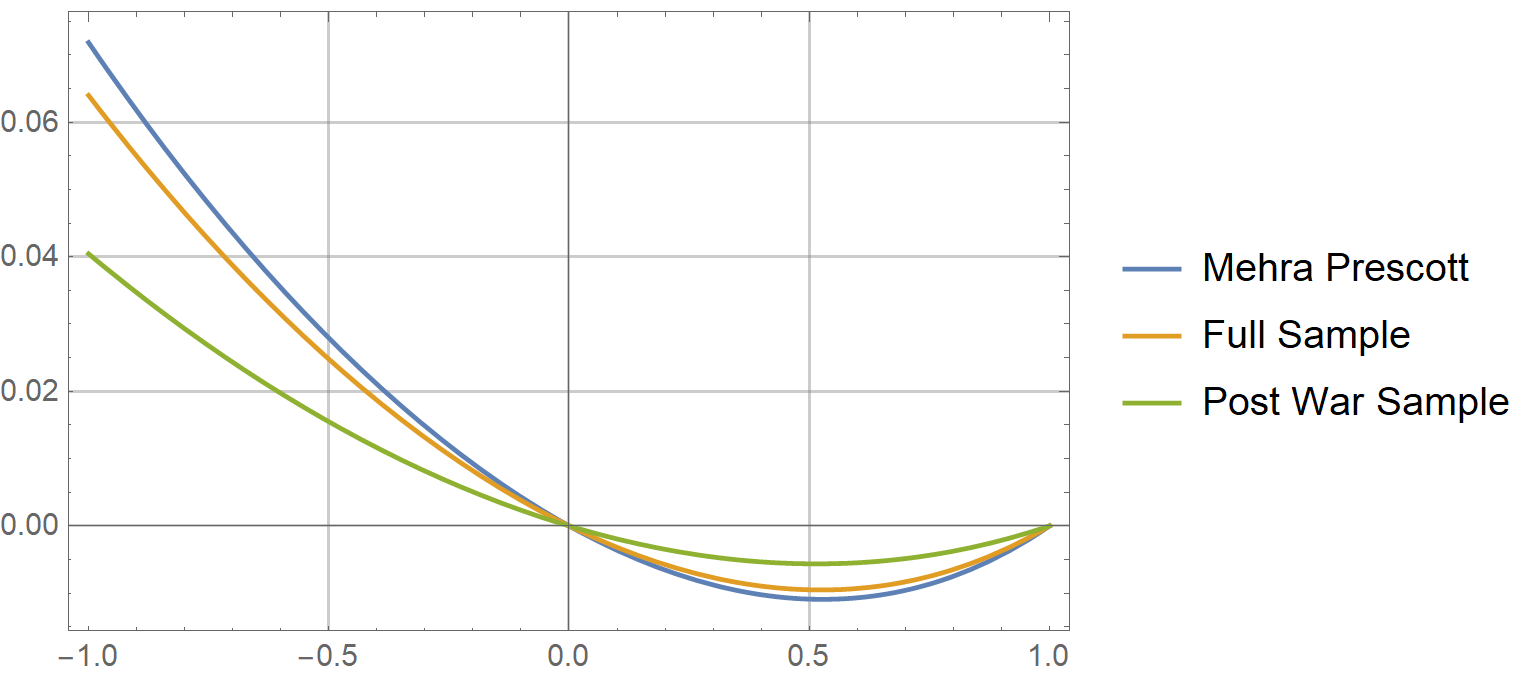
\includegraphics[width=0.75\textwidth]{risk_premium_rho.png}
 	\caption{Sensitivity of risk premium $\rho\in(-1, 1)$ for our various samples}
 	\label{fig:risk_premium_rho}
 \end{figure}
\end{enumerate}
  \begin{figure}[!htb]
	\centering
	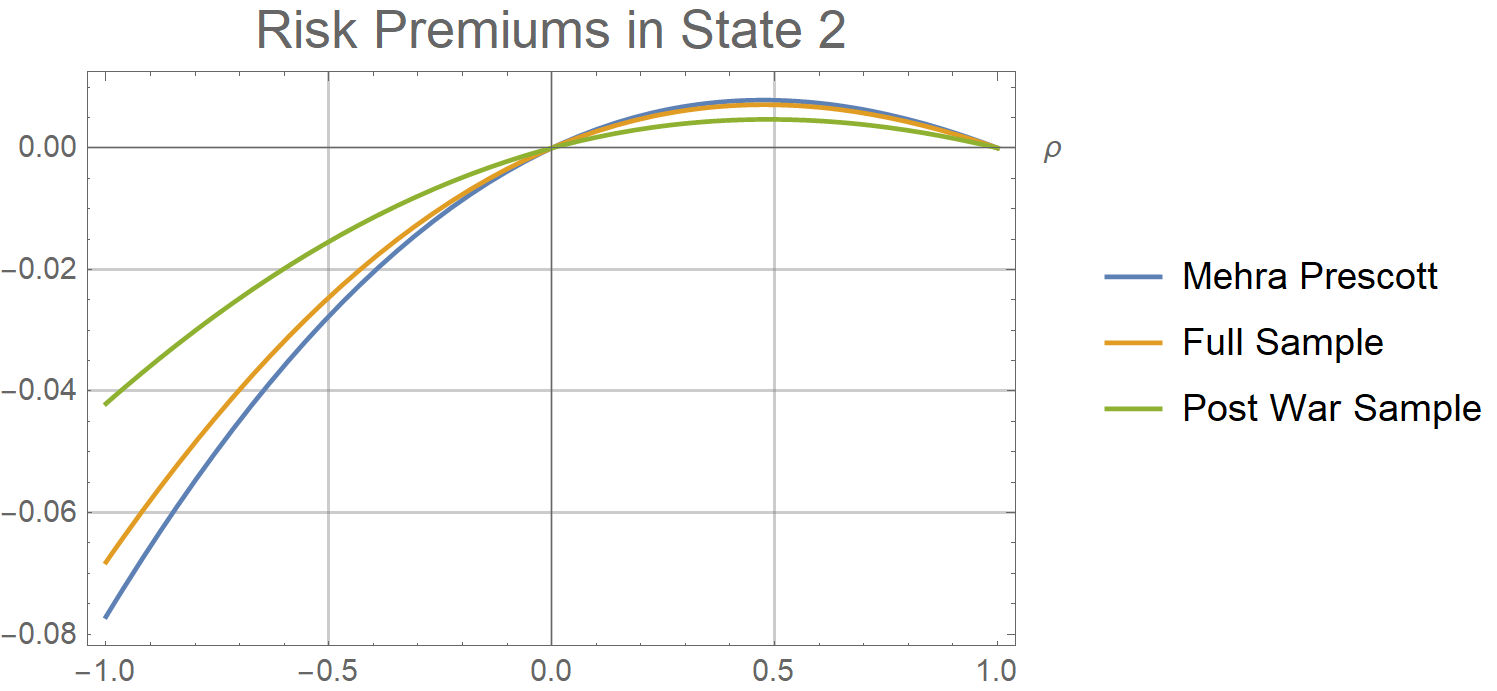
\includegraphics[width=0.75\textwidth]{risk_premium_rho_2.png}
	\caption{Sensitivity of risk premium $\rho\in(-1, 1)$ for our various samples}
	\label{fig:risk_premium_rho_2}
\end{figure}


\subsection*{c) Equity Premium}
\begin{enumerate}[I]
	\item A share of equity in this economy entitles the holder to the aggregate dividend in each period. Compute the equilibrium price dividend ration in state $i$. \\
	Let $P^e_i$ be the price of equity in state $i$and define $z_i \equiv \frac{P^e_i}{c_i}$. Then we have 
	\begin{equation}
	\begin{split}
		P^e_i &= \beta E_i\left[\lambda_{i'}^{-\alpha}(P^e_{i'} + c_{i'})\right]\\
		\implies \frac{P^e_i}{c_i}& = \beta E_i\left[\lambda_{i'}^{-\alpha}(\frac{P^e_{i'}}{c_{i'}} + 1)\frac{c_{i'}}{c_i}\right]\\
		&=\beta E_i\left[\lambda_{i'}^{1-\alpha}(\frac{P^e_{i'}}{c_{i'}} + 1)\right]\\
		&= \beta \sum_{j=1}^{2}\left[\pi_{ij}\lambda_j^{1-\alpha}\left(\frac{P^e_{j}}{c_{j}} + 1\right)\right]\\
		\implies z_i &=  \beta \sum_{j=1}^{2}\left[\pi_{ij}\lambda_j^{1-\alpha}\left(z_j + 1\right)\right]
	\end{split}
	\label{eq:price_dividend_ratio}
	\end{equation}
 Thus, the equilibrium price dividend ratio in each state is given by 	
	\begin{equation*}
		\begin{split}
		z_1 &=\beta\bigg(\pi_{11}\lambda_1^{1-\alpha}(z_1 + 1) + \pi_{12}\lambda_2^{1-\alpha}(z_2 + 1) \bigg)\\
		z_2& = \beta\bigg(\pi_{21}\lambda_1^{1-\alpha}(z_1 + 1) + \pi_{22}\lambda_2^{1-\alpha}(z_2 + 1) \bigg)\\
		\end{split}
	\end{equation*}
	This is a system of two equation and two unknowns, which imply the following price dividend ratios for the Mehra-Prescott parameters
	\begin{equation*}
		\begin{split}
		z_1 &= \frac{\beta  (\mu +\sigma ) \left((\rho +1) (\mu
			-\sigma )^{\alpha }+2 \beta  \rho  (\sigma -\mu
			)\right)-\beta  (\rho -1) (\mu -\sigma ) (\mu
			+\sigma )^{\alpha }}{(\mu +\sigma )^{\alpha }
			\left(2 (\mu -\sigma )^{\alpha }-\beta  (\rho +1)
			(\mu -\sigma )\right)+\beta  (\mu +\sigma ) \left(2
			\beta  \rho  (\mu -\sigma )-(\rho +1) (\mu -\sigma
			)^{\alpha }\right)}= 14.268\\
		z_2 & =  \frac{\beta  (\rho +1) (\mu -\sigma ) (\mu +\sigma
			)^{\alpha }+\beta  (\mu +\sigma ) \left((1-\rho )
			(\mu -\sigma )^{\alpha }+2 \beta  \rho  (\sigma
			-\mu )\right)}{(\mu +\sigma )^{\alpha } \left(2
			(\mu -\sigma )^{\alpha }-\beta  (\rho +1) (\mu
			-\sigma )\right)+\beta  (\mu +\sigma ) \left(2
			\beta  \rho  (\mu -\sigma )-(\rho +1) (\mu -\sigma
			)^{\alpha }\right)}=14.1436\\
		\end{split}
	\end{equation*}
	\item Compute the equilibrium returns on equity for each state. \\
	By homogeneity of degree one in consumption we have $P^e(i, c) = z_i c$. The period return if the current state is $(c, i)$ and next period is $(\lambda_jc, j)$ is 
	\begin{equation*}
		R^e_{ij} = \frac{P^e(\lambda_j c, j) + \lambda_j c}{P^e(c, i)} = \frac{\lambda_j(z_j + 1)}{z_i}
	\end{equation*}
	Thus, conditional on being in state $i$, the conditional expected equity return is 
	\begin{equation*}
	\begin{split}
			R^e(i) &= \sum_{j=1}^{2}\pi_{ij}R^e_{ij} = \pi_{i1}\frac{\lambda_1(z_1 + 1)}{z_i} + \pi_{i2}\frac{\lambda_2(z_2 + 1)}{z_i}\\
			R^e(1) &= \pi_{11}\frac{\lambda_1(z_1 + 1)}{z_1} + \pi_{12}\frac{\lambda_2(z_2 + 1)}{z_1}\\
			&=\frac{\beta  \rho  (\mu -\sigma ) (\mu +\sigma )
				\left((\rho +1) (\mu +\sigma )^{\alpha }-(\rho -1)
				(\mu -\sigma )^{\alpha }\right)-2 (\mu -\sigma
				)^{\alpha } (\mu +\sigma )^{\alpha } (\mu +\rho 
				\sigma )}{\beta  (\rho -1) (\mu -\sigma ) (\mu
				+\sigma )^{\alpha }+\beta  (\mu +\sigma ) \left(2
				\beta  \rho  (\mu -\sigma )-(\rho +1) (\mu -\sigma
				)^{\alpha }\right)}\\
			R^e(2) &= \pi_{21}\frac{\lambda_1(z_1 + 1)}{z_2} + \pi_{22}\frac{\lambda_2(z_2 + 1)}{z_2}\\
			&=\frac{\beta  \rho  (\mu -\sigma ) (\mu +\sigma )
				\left((\rho +1) (\mu -\sigma )^{\alpha }-(\rho -1)
				(\mu +\sigma )^{\alpha }\right)-2 (\mu -\sigma
				)^{\alpha } (\mu +\sigma )^{\alpha } (\mu -\rho 
				\sigma )}{\beta  (\mu +\sigma ) \left((\rho -1)
				(\mu -\sigma )^{\alpha }+2 \beta  \rho  (\mu
				-\sigma )\right)-\beta  (\rho +1) (\mu -\sigma )
				(\mu +\sigma )^{\alpha }}
	\end{split}
	\end{equation*}
	\item Using your results from the bond pricing section, compute the equilibrium excess returns on equity in each state. \\
	
	Define excess return as $R^x(i) = R^e(i) - R^f(i)$, where the risk free rate is given by $\frac{1}{b^1_i}$. Directly plugging in the result from the previous section and the bond pricing section and then simplifying, we get the following expressions
	\begin{equation*}
	\begin{split}
	R^x(1) &= \frac{\beta  \rho  (\mu -\sigma ) (\mu +\sigma )
		\left((\rho +1) (\mu +\sigma )^{\alpha }-(\rho -1)
		(\mu -\sigma )^{\alpha }\right)-2 (\mu -\sigma
		)^{\alpha } (\mu +\sigma )^{\alpha } (\mu +\rho 
		\sigma )}{\beta  (\rho -1) (\mu -\sigma ) (\mu
		+\sigma )^{\alpha }+\beta  (\mu +\sigma ) \left(2
		\beta  \rho  (\mu -\sigma )-(\rho +1) (\mu -\sigma
		)^{\alpha }\right)}\\
	&-\frac{2}{\beta  \left((\rho +1)
		(\mu +\sigma )^{-\alpha }-(\rho -1) (\mu -\sigma
		)^{-\alpha }\right)}\\
    R^x(2) &= \frac{\beta  \rho  (\mu -\sigma ) (\mu +\sigma )
    	\left((\rho +1) (\mu -\sigma )^{\alpha }-(\rho -1)
    	(\mu +\sigma )^{\alpha }\right)-2 (\mu -\sigma
    	)^{\alpha } (\mu +\sigma )^{\alpha } (\mu -\rho 
    	\sigma )}{\beta  (\mu +\sigma ) \left((\rho -1) (\mu
    	-\sigma )^{\alpha }+2 \beta  \rho  (\mu -\sigma
    	)\right)-\beta  (\rho +1) (\mu -\sigma ) (\mu +\sigma
    	)^{\alpha }}\\
    &-\frac{2}{\beta  \left((\rho +1) (\mu
    	+\sigma )^{-\alpha }-(\rho -1) (\mu -\sigma
    	)^{-\alpha }\right)}
	\end{split}
	\end{equation*}
		\begin{table}[!htbp] \centering 
		\caption{Price Dividend Ratios, Equity Returns, and Excess Returns} 
		\label{} 
		\begin{tabular}{@{\extracolsep{5pt}} ccccccc} 
			\\[-1.8ex]\hline 
			\hline \\[-1.8ex] 
			& $z_1$ & $z_2$ & $R^e_1$ & $R^e_2$ & $R^x_1$ & $R^x_2$  \\ 
			\hline \\[-1.8ex] 
			Mehra Prescott & $14.268$ & $14.436$ & $1.07$ & $1.10$ &0.003&0.025\\ 
			Full Sample & $31.84$ & $33.21$ & 1.08 & 1.02 &0.001&-0.05 \\ 
			Post War Sample & $32.17$ & 32.76 & 1.06 & 1.04 &0.004 &-0.025\\ 
			\hline \\[-1.8ex] 
		\end{tabular} 
	\end{table} 
	\item Use the stationary distribution for the Markov chain to compute the unconditional mean, standard deviation, and coefficient of first order autocorrelation for the excess returns on equity and the one period risk free interest rate. \\
	
	The long run mean of an arbitrary variable is defined as $E\left[x\right] = \sum_{i=1}^{2}\pi_i^*x_i$ and the variance is defined as $V(x) =  \sum_{i=1}^{2}\pi_i^*x_i^2 - (\sum_{i=1}^{2}\pi_i^*x_i)^2$, where $\pi_i^*$ denotes the probability from our long run distribution. Thus, for the excess returns we get the following
	
	\begin{equation*}
	\begin{split}
		E\left[R^x\right] &= 0.5 R^x(1) + 0.5 R^x(2)\\
		&= \frac{0.5 \left(\beta  (\mu -\sigma ) (\mu +\sigma )
			\left(-2 \left(\rho ^3+\rho \right) (\mu -\sigma
			)^{\alpha } (\mu +\sigma )^{\alpha }+(\rho -1)^2
			\rho  (\mu +\sigma )^{2 \alpha }+\rho  (\rho +1)^2
			(\mu -\sigma )^{2 \alpha }\right)+\right)}{\beta  \left((\rho +1) (\mu -\sigma
			)^{\alpha }-(\rho -1) (\mu +\sigma )^{\alpha
			}\right) \left((\mu +\sigma ) \left((\rho -1) (\mu
			-\sigma )^{\alpha }+2 \beta  \rho  (\mu -\sigma
			)\right)-(\rho +1) (\mu -\sigma ) (\mu +\sigma
			)^{\alpha }\right)}\\
			&+ \frac{0.5 \left(
			2 (\mu -\sigma
			)^{\alpha } \left((\mu -\sigma )^{\alpha }-(\mu
			+\sigma )^{\alpha }\right) (\mu +\sigma )^{\alpha }
			\left(-2 \mu  \rho +\rho ^2 \sigma +\sigma
			\right)\right)}{\beta  \left((\rho +1) (\mu -\sigma
			)^{\alpha }-(\rho -1) (\mu +\sigma )^{\alpha
			}\right) \left((\mu +\sigma ) \left((\rho -1) (\mu
			-\sigma )^{\alpha }+2 \beta  \rho  (\mu -\sigma
			)\right)-(\rho +1) (\mu -\sigma ) (\mu +\sigma
			)^{\alpha }\right)}\\
		&+\frac{0.5 \left(\beta  \rho 
			(\mu -\sigma ) (\mu +\sigma ) \left((\rho +1) (\mu
			+\sigma )^{\alpha }-(\rho -1) (\mu -\sigma
			)^{\alpha }\right)-2 (\mu -\sigma )^{\alpha } (\mu
			+\sigma )^{\alpha } (\mu +\rho  \sigma
			)\right)}{\beta  (\rho -1) (\mu -\sigma ) (\mu
			+\sigma )^{\alpha }+\beta  (\mu +\sigma ) \left(2
			\beta  \rho  (\mu -\sigma )-(\rho +1) (\mu -\sigma
			)^{\alpha }\right)}\\
		&-\frac{1}{\beta  \left((\rho
			+1) (\mu +\sigma )^{-\alpha }-(\rho -1) (\mu
			-\sigma )^{-\alpha }\right)}\\
		V(R^x) &=  0.5 (R^x(1))^2 + 0.5 (R^x(2))^2 +  (0.5 R^x(1) + 0.5 R^x(2))^2\\
	\end{split}
	\end{equation*}
   For the risk free rate, we get the following
   	\begin{equation*}
	   \begin{split}
	   E\left[R^f\right] &= 0.5 R^f(1) + 0.5 R^f(2)\\
	   &=\frac{1}{\beta  \left((\rho +1) (\mu +\sigma
	   	)^{-\alpha }-(\rho -1) (\mu -\sigma )^{-\alpha
	   	}\right)}+\frac{1}{\beta  \left((\rho +1) (\mu
	   	-\sigma )^{-\alpha }-(\rho -1) (\mu +\sigma
	   	)^{-\alpha }\right)}\\
	   V(R^f) &=  0.5 (R^f(1))^2 + 0.5 (R^f(2))^2 +  (0.5 R^f(1) + 0.5 R^f(2))^2\\	
	   \end{split}
   \end{equation*}
    To calculate the autocorrelation in state $i$ of a variable $X$, we need to compute 
    \begin{equation*}
    \begin{split}
    E_i\left[(X_i-E\left[X\right]) (X_j-E\left[X\right])\right] &=\pi_{i1}\left[(X_i-E\left[X\right]) (X_1-E\left[X\right])\right] +  \pi_{i2} \left[(X_i-E\left[X\right]) (X_2-E\left[X\right])\right]\\ 
    \end{split}
    \end{equation*}
    and then normalize this expression by the variance of the variable. The unconditional autocorrelation is then given by $\rho = \rho_1 \pi_1^* + \rho_2 \pi_2^*$
   	\begin{table}[!htbp] \centering 
   	\caption{Unconditional mean, standard deviation, and autocorrelations of excess return and risk free rate} 
   	\label{tab:erp_and_rf_puzzle} 
   	\begin{tabular}{@{\extracolsep{5pt}} ccccccc} 
   		\\[-1.8ex]\hline 
   		\hline \\[-1.8ex] 
   		& $E\left[R^x\right]$ & $\sigma\left(R^x\right)$ &$\rho(R^x)$& $E\left[R^f\right]$ &  $\sigma\left(R^f\right)$ &$\rho(R^f)$  \\ 
   		\hline \\[-1.8ex] 
   		Mehra Prescott & $0.013$ & $0.022$& & $0.087$ & $0.11$&\\ 
   		Full Sample& -0.03 & 0.045 & &0.05 & 0.05 \\ 
   		Post War Sample& -0.01 & 0.022 & &0.05& 0.01\\ 
   		\hline \\[-1.8ex] 
   	\end{tabular} 
   \end{table} 
\item The unconditional mean of the excess return on the US stock market over the last 100 years is about $6\%$ on annum. The unconditional mean of the risk free rate is close to zero. Inspecting Table \ref{tab:erp_and_rf_puzzle}, we see that the model implied equity risk premium is only $1.3\%$ and the risk free rate is $8.7\%$. Hence, we see both the equity risk premium puzzle (that the observed equity risk premium is much too high compared to the model) and the risk free rate puzzle (that the observed risk free rate is too low compared to the model). Additionally, we see that the model implied risk free rate is quite volatile, yet we observe fairly constant real risk free rates. \\
\item Derive the standard deviation of the risk free rate, the market rate, and the price-consumption ratio. How do these quantities fare relative to their data counterparts\\
For the standard deviation of the risk free rate, see Table 5. 
Once again we use our unconditional distribution $\Pi^*$ to calculate the variance of an arbitrary variable as $\sum_{i=1}^{2}\pi_i^*x_i^2 - (\sum_{i=1}^{2}\pi_i^*x_i)^2$
Using our previously derived expressions for $z$ and $R^e$, we get the following expressions for their variance
\begin{equation*}
	\resizebox{1.0\hsize}{!}{$
	V(z) = \frac{\beta ^2 \left(-2 (\mu
		-\sigma ) (\mu +\sigma
		)^{\alpha +1}
		\left(\left(\rho
		^2-2\right) (\mu -\sigma
		)^{\alpha }+4 \beta  \rho 
		(\mu -\sigma )\right)-8
		\beta  \rho  (\mu +\sigma
		)^2 (\mu -\sigma )^{\alpha
			+1}+\left(\rho ^2+2\right)
		(\mu +\sigma )^2 (\mu
		-\sigma )^{2 \alpha
		}+\left(\rho ^2+2\right)
		(\mu -\sigma )^2 (\mu
		+\sigma )^{2 \alpha }+8
		\beta ^2 \rho ^2 \left(\mu
		^2-\sigma
		^2\right)^2\right)}{\left((
		\mu +\sigma )^{\alpha }
		\left(2 (\mu -\sigma
		)^{\alpha }-\beta  (\rho
		+1) (\mu -\sigma
		)\right)+\beta  (\mu
		+\sigma ) \left(2 \beta 
		\rho  (\mu -\sigma )-(\rho
		+1) (\mu -\sigma )^{\alpha
		}\right)\right)^2}$
	}
\end{equation*}
and $V(R^e)$ is given by an extremely long expression.  

Plugging in our price consumption ratio and market rate to this formula, we get the following table 
		\begin{table}[!htbp] \centering 
	\caption{Standard deviation of market rate and price consumption ratio} 
	\begin{tabular}{@{\extracolsep{5pt}} ccccccc} 
		\\[-1.8ex]\hline 
		\hline \\[-1.8ex] 
		& $\sigma(z)$ & $\sigma(R^e)$   \\ 
		\hline \\[-1.8ex] 
		Mehra Prescott & $0.06$ & 0.01& \\ 
		Full Sample& 0.68 & 0.026 \\ 
		Post War Sample& 0.29 & 0.013 \\ 
		\hline \\[-1.8ex] 
	\end{tabular} 
\end{table}
Hence, the model implied standard deviations are both relatively low. 
	\end{enumerate}
\end{document}
